\documentclass{article}
\usepackage[utf8]{inputenc}
\usepackage[T1]{fontenc} % Use 8-bit encoding that has 256 glyphs
\usepackage{fourier} % Use the Adobe Utopia font for the document - comment this line to return to the LaTeX default
\usepackage[english]{babel} % English language/hyphenation
\usepackage{amsmath,amsfonts,amsthm} % Math packages
\usepackage{changepage}
\usepackage{graphicx}
\usepackage{sectsty} % Allows customizing section commands
\usepackage{qtree}
\allsectionsfont{\centering \normalfont\scshape} % Make all sections centered, the default font and small caps
\usepackage{algorithm2e}
\usepackage{fancyhdr} % Custom headers and footers
\usepackage{libertine}
\usepackage[svgnames]{xcolor}
\usepackage{framed}

\newcommand*\openquote{\makebox(25,-22){\scalebox{5}{``}}}%''
\newcommand*\closequote{\makebox(25,-22){\scalebox{5}{''}}}
\colorlet{shadecolor}{Azure}

\makeatletter
\newif\if@right
\def\shadequote{\@righttrue\shadequote@i}
\def\shadequote@i{\begin{snugshade}\begin{quote}\openquote}
\def\endshadequote{%
  \if@right\hfill\fi\closequote\end{quote}\end{snugshade}}
\@namedef{shadequote*}{\@rightfalse\shadequote@i}
\@namedef{endshadequote*}{\endshadequote}
\makeatother

\pagestyle{fancyplain} % Makes all pages in the document conform to the custom headers and footers
\fancyhead{} % No page header - if you want one, create it in the same way as the footers below
\fancyfoot[L]{} % Empty left footer
\fancyfoot[C]{} % Empty center footer
\fancyfoot[R]{\thepage} % Page numbering for right footer
\renewcommand{\headrulewidth}{0pt} % Remove header underlines
\renewcommand{\footrulewidth}{0pt} % Remove footer underlines
\setlength{\headheight}{13.6pt} % Customize the height of the header

\numberwithin{equation}{section} % Number equations within sections (i.e. 1.1, 1.2, 2.1, 2.2 instead of 1, 2, 3, 4)
\numberwithin{figure}{section} % Number figures within sections (i.e. 1.1, 1.2, 2.1, 2.2 instead of 1, 2, 3, 4)
\numberwithin{table}{section} % Number tables within sections (i.e. 1.1, 1.2, 2.1, 2.2 instead of 1, 2, 3, 4)
\def\changemargin#1#2{\list{}{\rightmargin#2\leftmargin#1}\item[]}
\let\endchangemargin=\endlist 
\setlength\parindent{0pt} % Removes all indentation from paragraphs - comment this line for an assignment with lots of text

%----------------------------------------------------------------------------------------
% TITLE SECTION
%----------------------------------------------------------------------------------------

\newcommand{\horrule}[1]{\rule{\linewidth}{#1}} % Create horizontal rule command with 1 argument of height

\title{
\large{\textsc{University of Victoria Computer Science}}\huge\\ [0pt] % Your university, school and/or department name(s)
\horrule{0.5pt}\\[0.4cm]
\textsc{Csc586A Theoretical Models\\Final Exam}\\
\author{Braden Simpson\\braden@uvic.ca\\V00685500}
\date{August 6, 2013}
}

\begin{document}

\maketitle % Print the title

\section{Question One}
\label{sec:one}
\subsection{Part A}
In this course, the theoretical model I chose to study most was for the project that Jordan and I did, and that model is the Abstract Syntax Tree (AST), more specifically, algorithms to find edit distances between them.  The AST is a tree represents the syntactic structure of source code, where each node is a construct (while, return, if etc.), leaves are variables, and branches are blocks of code.  See Appendix ~\ref{app:one} for an example.

By using these trees and the algorithms for edit distance, outlined by the fluri et al. \cite{fluri}, we were able to implement an algorithm for finding the changes between two ASTs.  I learned from the literature how to perform algorithms on these ASTs to find matching leaves, using levehnstein, n-grams, and other measures.

I also studied procedural generation and markov chains, but they weren't as in depth as the the trees.  I found the procedural generation algorithms such as L-Systems and Noise generation to be particularly interesting, especially because of their real-world use in video games and simulations.  Because the framework for L-Systems is so easy to learn, anybody can envision how they might be used in nature, which is sometimes hard to do when talking about theoretical models.

\subsection{Part B}
I used multiple different sources for my work, most of all the paper which helped us learn the algorithms required to perform tree edit distance calculations from fluri et al. \cite{fluri}.  As well I used different research on MSR conferences to learn how to analyze and interpret the data correctly, even as I was there this year, seeing the different ways people inetepret datasets has given me the insight required to critically assess what the data means, what inferences we can get, and more importantly, what we cannot get.  

\subsection{Part C}
\label{sec:q1c}
For this section I will do an example run of our algorithm for finding the change types in two ASTs for a file (before and after).  This will show how the algorithms are used to 


\begin{center}
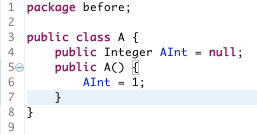
\includegraphics[width=0.5\linewidth]{codebefore}
\label{fig:cbefore}\\
The code for class A before a change.

\scriptsize
\begin{changemargin}{-0.5cm}{0cm} 
\Tree[.NAME(before.A) [.BODY\_DECLARATIONS  [.FieldDeclaration    [.Fragments \textit{A.Aint} ]
                                                                  [.Type \textit{java.lang.Integer} ]
                                                                  [.Modifiers \textit{public} ]]
                                            [.MethodDeclaration   [.Modifiers \textit{public} ]
                                                                  [.Name \textit{A.A()} ]
                                                                  [.Body [.Statement [.Expression [.LHS \textit{A.AInt} ]
                                                                                                  [.Operator \textit{'='} ]
                                                                                                  [.RHS [.ConstantValue \textit{1} ]]]]]]]]
\\
\end{changemargin}
\normalsize
The AST that corresponds to Figure ~\ref{fig:cbefore}
\end{center}

\begin{center}
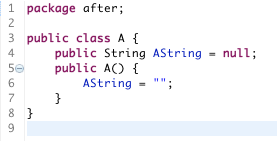
\includegraphics[width=0.5\linewidth]{codeafter}
\label{fig:cafter}\\
The code for class A after a change.

\scriptsize
\begin{changemargin}{-0.5cm}{0cm} 
\Tree[.NAME(after.A) [.BODY\_DECLARATIONS   [.FieldDeclaration    [.Fragments \textit{A.AString} ]
                                                                  [.Type \textit{java.lang.String} ]
                                                                  [.Modifiers \textit{public} ]]
                                            [.MethodDeclaration   [.Modifiers \textit{public} ]
                                                                  [.Name \textit{A.A()} ]
                                                                  [.Body [.Statement [.Expression [.LHS \textit{A.AString} ]
                                                                                                  [.Operator \textit{'='} ]
                                                                                                  [.RHS [.ConstantValue \textit{""} ]]]]]]]]
\\
\end{changemargin}
\normalsize
The AST that corresponds to Figure ~\ref{fig:cafter}
\end{center}


Once we have the two ASTs, we use methods in \cite{fluri} to match the nodes, using Levehnstein and n-gram similarity, to match the nodes.  Then we apply our rules, to find an edit script, namely what we need to do to get $Tree_1$ to $Tree_2$.  Using these rules: 

\begin{description}
  \item [\textbf{INSERT}]  $INST((l,v),y,k);$  Insert a new leaf node with label l and value v as the kth child of node y.
  \item [\textbf{DELETE}] $DEL(x);$ Delete node \emph{x} from it's parent.
  \item [\textbf{ALIGNMENT}]  $MOV(x, p(x), k);$ Node \emph{x} becomes the \emph{kth} child of \emph{p(x)}.
  \item [\textbf{MOVE}] $MOV(x, y, k), p(x) \neq y;$ Node \emph{x} becomes the \emph{kth} child of \emph{y}, and is deleted from \emph{p(x)}.
  \item [\textbf{UPDATE}] $UPD(x, val);$ Update \emph{v(x)} with \emph{val}, that is $val = v_{new}(x)$ and $v_{old}(x) \neq v_{new}(x)$.
\end{description}

We then result in the following changes. 
\begin{enumerate}
  \item DELETE - This is a delete into the method block of method \textit{A.a()}.  We then map this to our metric \textit{PUBLIC\_CHANGED\_INTERNAL\_METHODS}, since it's a change to the internals of a method.
  \item INSERT - The first is an insert into the method block of method \textit{A.a()}.  We then map this to our metric \textit{PUBLIC\_CHANGED\_INTERNAL\_METHODS}, since it's a change to the internals of a method.  The node was first deleted, and now it's inserted with a new value.
  \item DELETE - Removed the object state \textit{A.AInt}, causing a class field change, mapped to our metric \textit {PUBLIC\_CHANGED\_CLASSES}.
  \item INSERT - Added the object state \textit{A.AString}, causing a class field change, mapped to our metric \textit {PUBLIC\_CHANGED\_CLASSES}.
\end{enumerate}

We then do this for every file, for each commit, to sum up how many times each metric is changed.  We are then able to do our analysis on the data, interpreting it as a graph, in which we can make inferences about the trends of changes.  All of this work can be seen at our website\footnote{http://beast.segal.uvic.ca:3000}  

\footnotetext{Note that for Section~\ref{sec:q1c} I omitted a few nodes in the ASTs for simplicity, there are many that are generated by the JVM.}

\section{Question Two}
\label{sec:q2}
I am choosing the following papers for this question: \textit{A Density-Based Algorithm for Discovering Clusters in Large Spatial Dataases with Noise (DBSCAN)}~\cite{Ester96adensity-based}, and \textit{Semantic distance in WordNet: An experimental, application-oriented evaluation of five measures} ~\cite{Budanitsky01semanticdistance}.  

\subsection{DBSCAN}
This paper was a really good read and offered impressive results.  The authors first outline the scope of the research, which is clustering algorithms for spacial data. The authors first talk about what the clustering algorithms are, and come up with a list of requirements for a good clustering algorithm.  

In their abstract, the authors talk about the current best algorithm, and relate their proposed algorithm, DBSCAN against it, offering some instant validity.  The requirements for their clusting algorithm are outline, and they immediately give motivation for DBSCAN by saying that no other algorithms satisfy these requirements.  Furthermore, they say that DBSCAN is more efficient, robust, and functional, offering itself to a larger range of spatial databases.  

Section 2 of their paper discusses in detail all the leading algorithms according to their requirements, offering more evaluation of related work.  Then in Section 4, the authors introduce DBSCAN and finally in section 5 they use experimental data and benchmarks to validate their algorithm against the competitors in a simulation.  

This paper compared the runtime of each algorithm, and did many experiments to give a more general case to show an approximation of the running times of DBSCAN.

One of my main issues with the paper is that the authors compared DBSCAN against a different type of clustering algorithm (CLARANS), the two algorithms don't share any quantitative output, meaning that they have to be compared visually, which presents quite a large threat to the validity of the comparisons they do.  One thing I would have liked to see from the authors woulb be a comparison with an algorithm of the same type as DBSCAN, to avoid this problem.

Finally, the authors setup future work by considering objects other than point objects (polygons?) and they want to do more work with high dimensional feature spaces.  One thing they don't mention is comparison to any other related work or extra runtime evaluations.

\subsection{Semantic distance in WordNet}
This paper, by Budanitsky et al. presents definitions of \textit{semantic similarity} and more generally, \textit{relatedness} between words.  The authors then do an thorough evaluation of five different techniques for determining similarity.  

Firstly the authors introduce the concepts and describe their evaluation methods, which were as follows: 

\begin{enumerate}
  \item First a theoretical examination of a measure for desired properties (Wei 1993, Lin 1998) a good first coarse filter.
  \item Human judgements on the similarity, very hard to do because of time constraints, and can be hard to get subject-independant results.
  \item Thirdly, the authors use a Natural language parsing application to evaluate their measures, mixed with human evaluation.
\end{enumerate}

The authors used previous work by Rubenstein and Goodenough(1965), as well as Miller and Charles(1991), which used human subjects to rank the similarity between a set of 65 pairs of words.  The authors implemented the five measures, on the 65 pairs of words to compare how well their implementations were to the human judgement.  

The authors are critical of their method, saying that in the perfect world, they would have a really large human judged test set, but that is a very difficult task to accomplish.  They then talk about methodological problems with the prior human studies.

\begin{shadequote}
It was implicit in the Rubenstein–Goodenough and Miller–Charles experiments that subjects were to use the dominant sense of the target words. But what we are really interested in is the relationship between the concepts for which the words are merely surrogates; the human judgments that we need are of the relatedness of word-senses, not words. So the experimental situation would need to set up contexts that bias the sense selection for each target word and yet don’t bias the subject’s judgment of their a priori relationship, an almost self-contradictory situation.\par\emph{Budanitsky et al.~\cite{Budanitsky01semanticdistance}}
\end{shadequote}

Next the authors evaluated the measures using the property of \textit{malapropism} which is, spelling errors in open class words.  The way the authors performed the tests was to do more simulations on 500 articles from the \textit{Wall Street Journal}, with 107,233 unique words, 1408 of which were malapropisms.  

The authors then did an retrospective analysis of their results in the conclusions which showed their critique of their own algorithms, and insights as to which algorithm is best, and why.  They also talked about their limitations, and problems of the study.

\section{Question 3}
For question three, the two papers I am choosing as \textit{optimization} papers are \textit{Partial Parsing via Finite-State Cascades}~\cite{Abney:1996:PPV:974697.974705}, and \textit{Network Coding Meets TCP: Theory and Implementation}

\subsection{Partial Parsing}
This paper was the first thing that came to my mind in terms of optimization.  To begin, the paper is performing a task that is not novel, so the paper's contribution must be something which improves, sheds new light on, or modifies an existing method.  

This paper introduces a new method of parsing through unstructured text such as human language.  It does so by using a method of cascading finite state transducers which transform text based on some grammars.  The authors evaluate these methods with an extensive set of language, with both german and english.  

The reason why this paper \textit{optimizes}, is because they have quantitative measures of how fast the traditional parsers can run (words/second), and then use that as their baseline for their new method.  This gives them a goal to beat.  The properties being optimized in this case are speed and accuracy, and the method these authors provide is measured for both.  The speed is optimized and shown to be around 3000:1 increase in words/second.  And the table below (taken from the paper ~\cite{Abney:1996:PPV:974697.974705}) shows the optimization in accuracy. 

\begin{center}
  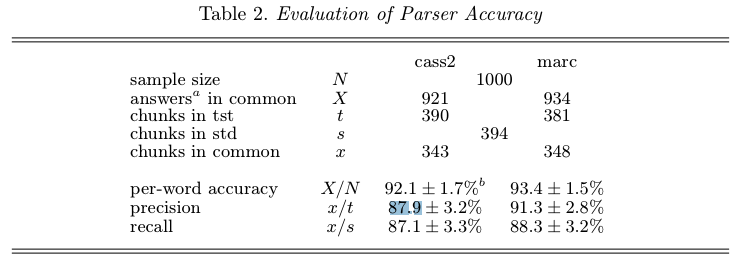
\includegraphics[width=\textwidth]{partialaccuracy}
\end{center}

The importance of both speed and accuracy in parsing of unstructured text is paramount, without quick, accurate parsers such as the ones proposed in this paper, and further studies, we would not have the technology like google, siri, many data-mining techniques, and much more.

\subsection{}

\appendix
\section{Abstract Syntax Trees}
\label{app:one}
\scriptsize
\begin{changemargin}{-4cm}{0cm} 
\Tree[.{statement name} [.while [.{compare op: $\neq$}  [\textit{variable: b} ]
                                                        [\textit{constant: 0} ]]
                                [.branch [.{compare op >} [\textit{variable: a} ]
                                                          [\textit{variable: b} ]]
                                          [.assign         [\textit{variable: a} ]
                                                          [.{op -}  [\textit{variable: a} ]
                                                                    [\textit{variable: b} ]]]
                                          [.assign        [\textit{variable: b} ]
                                                          [.{op -}  [\textit{variable: b} ]
                                                                    [\textit{variable: a} ]]]]]
                        [.return !\qsetw{10cm} \textit{variable: a} ]]
\end{changemargin} 
\normalsize
\begin{algorithm}[H]
 \SetAlgoLined
 \KwData{An abstract syntax tree with matching psuedocode for Euclidean Algorithm.  Taken from the wikipedia entry \footnote{http://en.wikipedia.org/wiki/Abstract\_syntax\_tree}}
 \While{b $\neq$ 0}{
  \eIf{a > b}{
    a = a - b      
  }{
    b = b - a
  }
}
return a
\end{algorithm}
\bibliographystyle{IEEEtran}
\bibliography{final} 
\end{document}